\documentclass[aspectratio=169,11pt]{beamer}
\usepackage{../../../shared/theme/esmad_beamer_theme}

% Shared canonical Beamer shell is provided by esmad_beamer_theme.

% Packages
\usepackage{amsmath,amsthm,amssymb}
\usepackage{graphicx}
\usepackage{tikz}
\usepackage{algorithm,algorithmic}
\usepackage{booktabs}
\usepackage{multirow}
\usepackage{xcolor}
\usepackage{listings}
\usepackage{subcaption}
\usepackage{hyperref}

% TikZ libraries for DAGs
\usetikzlibrary{arrows,positioning,calc}

% Custom colors
\definecolor{navyblue}{RGB}{0,32,96}
\definecolor{crimson}{RGB}{178,34,52}
\definecolor{forest}{RGB}{34,139,34}
\definecolor{gold}{RGB}{255,215,0}
\definecolor{purple}{RGB}{128,0,128}

% Code listing settings
\lstset{
    language=Python,
    basicstyle=\ttfamily\small,
    keywordstyle=\color{navyblue}\bfseries,
    commentstyle=\color{forest}\itshape,
    stringstyle=\color{crimson},
    numbers=left,
    numberstyle=\tiny\color{gray},
    stepnumber=1,
    tabsize=2,
    showstringspaces=false,
    breaklines=true,
    frame=single,
    rulecolor=\color{gray!30}
}

% Title information
\title[Causal Inference]{Causal Inference for Data Scientists}
\subtitle{From Correlation to Causation}
\date{\today}

% Custom commands
\newcommand{\E}{\mathbb{E}}
\newcommand{\Var}{\text{Var}}
\newcommand{\Cov}{\text{Cov}}
\newcommand{\indep}{\perp\!\!\!\perp}
\newcommand{\nindep}{\not\!\perp\!\!\!\perp}
\newcommand{\btheta}{\boldsymbol{\theta}}
\newcommand{\bx}{\mathbf{x}}
\newcommand{\by}{\mathbf{y}}
\newcommand{\bmu}{\boldsymbol{\mu}}
\newcommand{\bSigma}{\boldsymbol{\Sigma}}
\newcommand{\argmin}{\text{argmin}}
\newcommand{\argmax}{\text{argmax}}
\newcommand{\Real}{\mathbb{R}}
% \do is a primitive command in TeX; define a safe math operator instead
\DeclareMathOperator{\doo}{do}

\begin{document}

% Title slide
\begin{frame}
\titlepage
\end{frame}

% Learning goals
\begin{frame}{Learning Goals}
\begin{itemize}
\item distinguish predictive association from causal effects using potential outcomes and DAGs;
\item select identification strategies (RCT, IV, RDD, DiD, matching) based on assumptions and data constraints;
\item run practical diagnostics and communicate limitations transparently in policy and business settings.
\end{itemize}
\end{frame}

% Table of contents
\begin{frame}{Outline}
\tableofcontents
\end{frame}

\section{The Causal Revolution in Data Science}

\begin{frame}{Correlation vs Causation: The Fundamental Distinction}
\begin{columns}
\begin{column}{0.6\textwidth}
\begin{block}{Central question}
A causal analysis asks how an outcome would change under a well-defined intervention or treatment assignment, relative to an explicit counterfactual comparison.
\end{block}

\vspace{0.3cm}
\textbf{The Problem with Pure Prediction:}
\begin{itemize}
\item \textcolor{crimson}{Association $\neq$ Causation}: High correlation doesn't mean one causes the other
\item \textcolor{crimson}{Confounding}: Hidden variables affect both cause and effect
\item \textcolor{crimson}{Spurious correlations}: Random chance or third variables
\item \textcolor{crimson}{Simpson's paradox}: Correlations reverse when conditioning
\end{itemize}

\vspace{0.3cm}
\textbf{Why Causation Matters:}
\begin{itemize}
\item \textcolor{forest}{Decision making}: What happens if we intervene?
\item \textcolor{forest}{Policy evaluation}: Did the treatment work?
\item \textcolor{forest}{Counterfactuals}: What would have happened?
\item \textcolor{forest}{Generalization}: Understanding transfers across contexts
\end{itemize}
\end{column}
\begin{column}{0.4\textwidth}
\begin{figure}
\centering
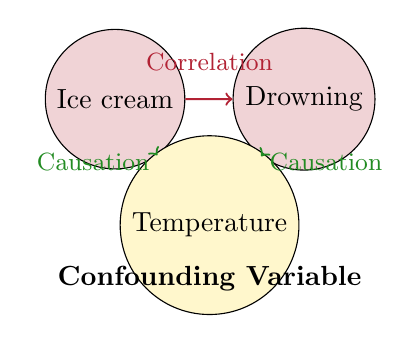
\begin{tikzpicture}[scale=0.8]
% Spurious correlation example
\node[draw, circle, fill=crimson!20] (ice) at (0,2) {Ice cream};
\node[draw, circle, fill=crimson!20] (drowning) at (3,2) {Drowning};
\node[draw, circle, fill=gold!20] (temp) at (1.5,0) {Temperature};

% Spurious correlation
\draw[->, thick, crimson] (ice) -- (drowning);
\node[above] at (1.5,2.3) {\color{crimson}\small Correlation};

% True causal relationships
\draw[->, thick, forest] (temp) -- (ice);
\draw[->, thick, forest] (temp) -- (drowning);
\node[left] at (0.7,1) {\color{forest}\small Causation};
\node[right] at (2.3,1) {\color{forest}\small Causation};

\node[below] at (1.5,-0.5) {\textbf{Confounding Variable}};
\end{tikzpicture}
\end{figure}
\begin{alertblock}{The Causal Hierarchy}
\begin{enumerate}
\item \textbf{Association}: $P(Y|X)$
\item \textbf{Intervention}: $P(Y|\doo(X))$
\item \textbf{Counterfactuals}: $P(Y_x|X',Y')$
\end{enumerate}
\end{alertblock}
\end{column}
\end{columns}
\end{frame}

\begin{frame}{Famous Examples of Causal Confusion}
\begin{table}
\centering
\small
\begin{tabular}{p{3cm}p{4cm}p{4cm}}
\toprule
\textbf{Spurious Correlation} & \textbf{What People Concluded} & \textbf{Real Explanation} \\
\midrule
Chocolate consumption vs Nobel prizes & Chocolate makes you smarter & Wealth enables both luxuries and research \\
\midrule
Ice cream sales vs crime rates & Ice cream causes crime & Hot weather increases both \\
\midrule
Facebook friends vs longevity & Social media extends life & Social people live longer and use Facebook \\
\midrule
Stork populations vs birth rates & Storks deliver babies & Rural areas have both more storks and higher birth rates \\
\midrule
Shoe size vs reading ability & Big feet help reading & Age affects both shoe size and reading skills \\
\bottomrule
\end{tabular}
\end{table}

\begin{columns}
\begin{column}{0.5\textwidth}
\textbf{Business Implications:}
\begin{itemize}
\item \textcolor{crimson}{Wrong investments}: Correlation-based decisions
\item \textcolor{crimson}{Failed interventions}: Treating symptoms, not causes
\item \textcolor{crimson}{Wasted resources}: Ineffective policies
\item \textcolor{crimson}{Opportunity costs}: Missing real causal factors
\end{itemize}
\end{column}
\begin{column}{0.5\textwidth}
\textbf{The Data Science Challenge:}
\begin{itemize}
\item Most ML focuses on prediction ($P(Y|X)$)
\item Business needs intervention effects ($P(Y|\do(X))$)
\item Observational data is riddled with confounders
\item Randomized experiments aren't always possible
\end{itemize}
\end{column}
\end{columns}

\begin{alertblock}{Key Insight}
Causal inference is the bridge between data science and evidence-based decision making.
\end{alertblock}
\end{frame}

\begin{frame}{The Potential Outcomes Framework}
\textbf{Rubin Causal Model:} Formalize causation through potential outcomes.

\begin{columns}
\begin{column}{0.5\textwidth}
\textbf{Setup:}
\begin{itemize}
\item Units: $i = 1, 2, \ldots, n$
\item Treatment: $T_i \in \{0, 1\}$
\item Potential outcomes: 
  \begin{itemize}
  \item $Y_i(1)$: Outcome if treated
  \item $Y_i(0)$: Outcome if not treated
  \end{itemize}
\item Observed outcome: $Y_i = T_i Y_i(1) + (1-T_i) Y_i(0)$
\end{itemize}

\textbf{Individual Treatment Effect:}
\[\tau_i = Y_i(1) - Y_i(0)\]

\textbf{The Fundamental Problem:}
We can never observe both $Y_i(1)$ and $Y_i(0)$ for the same unit!
\end{column}
\begin{column}{0.5\textwidth}
\textbf{Average Treatment Effect (ATE):}
\[\tau = \E[Y_i(1) - Y_i(0)] = \E[Y_i(1)] - \E[Y_i(0)]\]

\textbf{What We Can Observe:}
\begin{align}
\E[Y|T=1] - \E[Y|T=0] &= \E[Y(1)|T=1] - \E[Y(0)|T=0]\\
&= \underbrace{\E[Y(1)] - \E[Y(0)]}_{\text{ATE}} \\
&\quad + \underbrace{\E[Y(0)|T=1] - \E[Y(0)|T=0]}_{\text{Selection Bias}}
\end{align}

\begin{alertblock}{Selection Bias}
The difference in outcomes would exist even without treatment, due to systematic differences between treated and untreated groups.
\end{alertblock}
\end{column}
\end{columns}

\textbf{Goal:} Identify conditions under which \(\mathbb{E}[Y\mid T=1] - \mathbb{E}[Y\mid T=0] = \tau\).
\end{frame}

\section{Causal Graphs and DAGs}

\begin{frame}{Directed Acyclic Graphs (DAGs)}
\textbf{Tool:} Represent causal assumptions using directed graphs.

\begin{columns}
\begin{column}{0.6\textwidth}
\textbf{DAG Components:}
\begin{itemize}
\item \textbf{Nodes}: Variables (observed and unobserved)
\item \textbf{Directed edges}: Direct causal relationships
\item \textbf{Paths}: Sequences of edges
\item \textbf{No cycles}: Acyclic assumption
\end{itemize}

\vspace{0.3cm}
\textbf{Three Fundamental Structures:}

\begin{enumerate}
\item \textbf{Chain}: $X \to Z \to Y$ (mediation)
\item \textbf{Fork}: $X \leftarrow Z \rightarrow Y$ (confounding)
\item \textbf{Collider}: $X \rightarrow Z \leftarrow Y$ (selection bias)
\end{enumerate}

\vspace{0.3cm}
\textbf{d-separation}: Paths are blocked by conditioning on certain variables.
\end{column}
\begin{column}{0.4\textwidth}
\begin{figure}
\centering
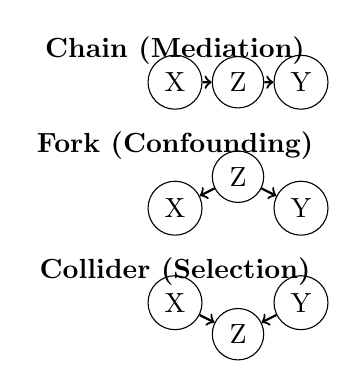
\begin{tikzpicture}[scale=0.8]
% Chain
\node at (0,3) {\textbf{Chain (Mediation)}};
\node[draw, circle] (X1) at (0,2.5) {X};
\node[draw, circle] (Z1) at (1,2.5) {Z};
\node[draw, circle] (Y1) at (2,2.5) {Y};
\draw[->, thick] (X1) -- (Z1);
\draw[->, thick] (Z1) -- (Y1);

% Fork
\node at (0,1.5) {\textbf{Fork (Confounding)}};
\node[draw, circle] (Z2) at (1,1) {Z};
\node[draw, circle] (X2) at (0,0.5) {X};
\node[draw, circle] (Y2) at (2,0.5) {Y};
\draw[->, thick] (Z2) -- (X2);
\draw[->, thick] (Z2) -- (Y2);

% Collider
\node at (0,-0.5) {\textbf{Collider (Selection)}};
\node[draw, circle] (X3) at (0,-1) {X};
\node[draw, circle] (Y3) at (2,-1) {Y};
\node[draw, circle] (Z3) at (1,-1.5) {Z};
\draw[->, thick] (X3) -- (Z3);
\draw[->, thick] (Y3) -- (Z3);
\end{tikzpicture}
\end{figure}

\begin{block}{d-separation Rules}
\begin{itemize}
\item \textbf{Chain/Fork}: Blocked by conditioning on middle node
\item \textbf{Collider}: Blocked unless we condition on collider or its descendants
\end{itemize}
\end{block}
\end{column}
\end{columns}

\textbf{Pearl's Causal Hierarchy}: DAGs enable us to move from association to intervention to counterfactuals.
\end{frame}

\begin{frame}{The Backdoor Criterion}
\textbf{Goal:} Identify when we can estimate causal effects from observational data.

\begin{columns}
\begin{column}{0.5\textwidth}
\begin{definition}[Backdoor Criterion]
A set of variables $Z$ satisfies the backdoor criterion relative to $(X, Y)$ if:
\begin{enumerate}
\item No node in $Z$ is a descendant of $X$
\item $Z$ blocks every backdoor path from $X$ to $Y$
\end{enumerate}
\end{definition}

\textbf{Backdoor path}: Any path from $X$ to $Y$ that starts with an arrow into $X$.

\textbf{Backdoor Adjustment Formula:}
\[P(Y = y | \doo(X = x)) = \sum_z P(Y = y | X = x, Z = z) P(Z = z)\]
\[P(Y = y | \do(X = x)) = \sum_z P(Y = y | X = x, Z = z) P(Z = z)\]
\textbf{In expectation:}
\[\E[Y | \doo(X = x)] = \sum_z \E[Y | X = x, Z = z] P(Z = z)\]
\[\E[Y | \do(X = x)] = \sum_z \E[Y | X = x, Z = z] P(Z = z)\]
\end{column}
\begin{column}{0.5\textwidth}
\begin{figure}
\centering
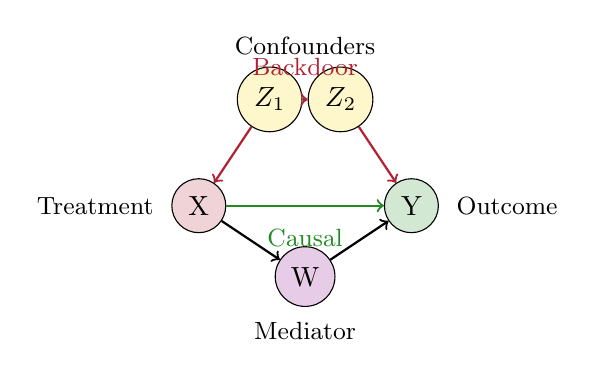
\begin{tikzpicture}[scale=0.9]
% Example DAG with backdoor path
\node[draw, circle, fill=crimson!20] (X) at (0,1) {X};
\node[draw, circle, fill=forest!20] (Y) at (3,1) {Y};
\node[draw, circle, fill=gold!20] (Z1) at (1,2.5) {$Z_1$};
\node[draw, circle, fill=gold!20] (Z2) at (2,2.5) {$Z_2$};
\node[draw, circle, fill=purple!20] (W) at (1.5,0) {W};

% Causal path
\draw[->, thick, forest] (X) -- (Y);
\node[below] at (1.5,0.8) {\color{forest}\small Causal};

% Backdoor path
\draw[->, thick, crimson] (Z1) -- (X);
\draw[->, thick, crimson] (Z1) -- (Z2);
\draw[->, thick, crimson] (Z2) -- (Y);
\node[above] at (1.5,2.7) {\color{crimson}\small Backdoor};

% Mediator
\draw[->, thick] (X) -- (W);
\draw[->, thick] (W) -- (Y);

% Annotations
\node[left] at (-0.5,1) {\small Treatment};
\node[right] at (3.5,1) {\small Outcome};
\node[above] at (1.5,3) {\small Confounders};
\node[below] at (1.5,-0.5) {\small Mediator};
\end{tikzpicture}
\end{figure}

\textbf{To estimate causal effect:}
\begin{itemize}
\item \textcolor{forest}{Include}: $Z_1, Z_2$ (block backdoor)
\item \textcolor{crimson}{Exclude}: $W$ (mediator, descendant of $X$)
\end{itemize}

\begin{alertblock}{Key Insight}
Controlling for the "right" variables enables causal identification from observational data.
\end{alertblock}
\end{column}
\end{columns}
\end{frame}

\begin{frame}{DAGs: What the Graph Encodes}
\begin{itemize}
  \item Nodes represent variables; directed edges encode assumed direct causal relationships.
  \item A DAG is a formal statement of assumptions, not a pattern learned automatically from observational correlations.
  \item For the effect of Education on Income, plausible common causes such as Family Background, Ability, and Location can open backdoor paths.
  \item Post-treatment variables such as Experience may mediate part of the effect and should not be adjusted for when estimating the total effect.
\end{itemize}

\begin{alertblock}{Adjustment principle}
Choose covariates that block noncausal backdoor paths without conditioning on descendants of treatment or colliders that would create new biasing paths.
\end{alertblock}
\end{frame}

\begin{frame}[fragile]{DAGs in Python: Represent the Assumptions}
\begin{lstlisting}[style=code,basicstyle=\ttfamily\small]
import networkx as nx

G = nx.DiGraph()
G.add_edges_from([
    ("Family_Background", "Education"),
    ("Family_Background", "Income"),
    ("Ability", "Education"),
    ("Ability", "Income"),
    ("Location", "Education"),
    ("Location", "Income"),
    ("Education", "Experience"),
    ("Experience", "Income"),
    ("Education", "Income"),
])

assert nx.is_directed_acyclic_graph(G)
\end{lstlisting}

\begin{block}{What this code does}
NetworkX is useful for representing and visualizing the assumed graph. A hand-written path checker is not a substitute for a correct d-separation or adjustment-set algorithm.
\end{block}
\end{frame}

\begin{frame}{DAGs: From Graph to Adjustment Set}
\begin{enumerate}
  \item Draw the causal graph from substantive knowledge and design information.
  \item Identify all backdoor paths from treatment to outcome.
  \item Find a sufficient adjustment set that blocks those paths.
  \item Check that the set does not include treatment descendants or open collider paths.
  \item Perform sensitivity analysis because unmeasured variables are absent from the observed graph by construction.
\end{enumerate}

\begin{block}{Example}
For the graph shown here, Family Background, Ability, and Location are candidate pre-treatment common causes. Experience is downstream of Education and is inappropriate when the target is the total effect.
\end{block}

\begin{alertblock}{Remember}
DAGs make identification assumptions explicit. They do not validate those assumptions by themselves.
\end{alertblock}
\end{frame}

\section{Identification Strategies}

\begin{frame}{Randomized Controlled Trials: The Gold Standard}
\textbf{Why Randomization Works:} Breaks the link between treatment and confounders.

\begin{columns}
\begin{column}{0.5\textwidth}
\textbf{Randomization Ensures:}
\begin{align}
Y_i(1), Y_i(0) \indep T_i
\end{align}

This means:
\begin{align}
\E[Y(1)|T=1] &= \E[Y(1)]\\
\E[Y(0)|T=0] &= \E[Y(0)]
\end{align}

Therefore:
\begin{align}
\text{ATE} &= \E[Y|T=1] - \E[Y|T=0]
\end{align}

\textbf{No confounding bias!}

\vspace{0.3cm}
\textbf{RCT Advantages:}
\begin{itemize}
\item Unbiased estimates
\item Simple analysis
\item High internal validity
\item Clear causal interpretation
\end{itemize}
\end{column}
\begin{column}{0.5\textwidth}
\begin{figure}
\centering
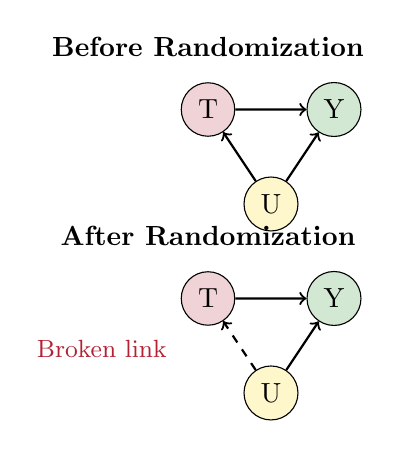
\begin{tikzpicture}[scale=0.8]
% Before randomization
\node at (0,3) {\textbf{Before Randomization}};
\node[draw, circle, fill=crimson!20] (T1) at (0,2) {T};
\node[draw, circle, fill=forest!20] (Y1) at (2,2) {Y};
\node[draw, circle, fill=gold!20] (U1) at (1,0.5) {U};

\draw[->, thick] (U1) -- (T1);
\draw[->, thick] (U1) -- (Y1);
\draw[->, thick] (T1) -- (Y1);

% After randomization
\node at (0,0) {\textbf{After Randomization}};
\node[draw, circle, fill=crimson!20] (T2) at (0,-1) {T};
\node[draw, circle, fill=forest!20] (Y2) at (2,-1) {Y};
\node[draw, circle, fill=gold!20] (U2) at (1,-2.5) {U};

\draw[->, thick, dashed] (U2) -- (T2);
\draw[->, thick] (U2) -- (Y2);
\draw[->, thick] (T2) -- (Y2);

\node[left] at (-0.5,-1.8) {\color{crimson}\small Broken link};
\end{tikzpicture}
\end{figure}

\textbf{When RCTs Are Limited:}
\begin{itemize}
\item \textcolor{crimson}{Ethical constraints}: Harmful treatments
\item \textcolor{crimson}{Practical constraints}: Cost, time, feasibility
\item \textcolor{crimson}{External validity}: Lab vs real world
\item \textcolor{crimson}{Compliance issues}: Not everyone follows assignment
\end{itemize}

\begin{alertblock}{The Gap}
Most business/policy questions can't be answered with RCTs. We need methods for observational data.
\end{alertblock}
\end{column}
\end{columns}
\end{frame}

\begin{frame}[fragile]{Instrumental Variables: Finding Natural Experiments}
\textbf{Idea:} Use a variable that affects treatment but not outcome directly.

\begin{columns}
\begin{column}{0.55\textwidth}
\begin{definition}[Instrumental Variable]
$Z$ is an instrument for $X \rightarrow Y$ if:
\begin{enumerate}
\item \textbf{Relevance}: $Z$ affects $X$ (strong first stage)
\item \textbf{Exclusion}: $Z$ affects $Y$ only through $X$
\item \textbf{Independence}: $Z$ is as-good-as-randomly assigned
\end{enumerate}
\end{definition}

\begin{lstlisting}[basicstyle=\ttfamily\tiny]
import numpy as np
import pandas as pd
from sklearn.linear_model import LinearRegression
from scipy import stats
import statsmodels.api as sm
from statsmodels.sandbox.regression.gmm import IV2SLS

# Simulate data with endogeneity
np.random.seed(42)
n = 1000

# Unobserved confounder
U = np.random.randn(n)

# Instrument (randomly assigned)
Z = np.random.binomial(1, 0.5, n)

# Treatment (affected by instrument and confounder)
X = 0.5 * Z + 0.3 * U + np.random.randn(n) * 0.2

# Outcome (affected by treatment and confounder)
Y = 1.0 * X + 0.4 * U + np.random.randn(n) * 0.3

df = pd.DataFrame({'Y': Y, 'X': X, 'Z': Z, 'U': U})

print("True causal effect: 1.0")

# Naive OLS (biased due to confounding)
ols = LinearRegression().fit(df[['X']], df['Y'])
ols_coef = ols.coef_[0]
print(f"OLS estimate: {ols_coef:.3f}")

# Two-Stage Least Squares (2SLS)
# First stage: X ~ Z
first_stage = LinearRegression().fit(df[['Z']], df['X'])
X_hat = first_stage.predict(df[['Z']])

# Check first-stage strength
f_stat = (first_stage.score(df[['Z']], df['X']) * (n-2)) / (1 - first_stage.score(df[['Z']], df['X']))
print(f"First-stage F-statistic: {f_stat:.2f}")

# Second stage: Y ~ X_hat
second_stage = LinearRegression().fit(X_hat.reshape(-1, 1), df['Y'])
iv_coef = second_stage.coef_[0]
print(f"IV estimate: {iv_coef:.3f}")

# Using statsmodels for proper inference
iv_model = IV2SLS(df['Y'], df[['X']], df[['Z']], df[['Z']]).fit()
print(f"IV (statsmodels): {iv_model.params[0]:.3f} ({iv_model.pvalues[0]:.3f})")

# Reduced form (effect of Z on Y)
reduced_form = LinearRegression().fit(df[['Z']], df['Y'])
rf_coef = reduced_form.coef_[0]

# Manual IV calculation: reduced form / first stage
manual_iv = rf_coef / first_stage.coef_[0]
print(f"Manual IV calculation: {manual_iv:.3f}")
\end{lstlisting}
\end{column}
\begin{column}{0.45\textwidth}
\begin{figure}
\centering
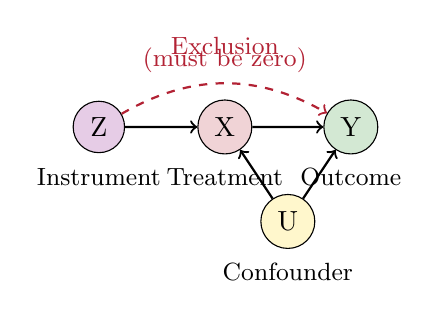
\begin{tikzpicture}[scale=0.8]
\node[draw, circle, fill=purple!20] (Z) at (0,2) {Z};
\node[draw, circle, fill=crimson!20] (X) at (2,2) {X};
\node[draw, circle, fill=forest!20] (Y) at (4,2) {Y};
\node[draw, circle, fill=gold!20] (U) at (3,0.5) {U};

% Valid arrows
\draw[->, thick] (Z) -- (X);
\draw[->, thick] (X) -- (Y);
\draw[->, thick] (U) -- (X);
\draw[->, thick] (U) -- (Y);

% Invalid arrow (exclusion restriction)
\draw[->, thick, dashed, crimson] (Z) to[bend left] (Y);
\node[above] at (2,3) {\color{crimson}\small Exclusion};
\node[above] at (2,2.7) {\color{crimson}\small (must be zero)};

\node[below] at (0,1.5) {\small Instrument};
\node[below] at (2,1.5) {\small Treatment};
\node[below] at (4,1.5) {\small Outcome};
\node[below] at (3,0) {\small Confounder};
\end{tikzpicture}
\end{figure}

\textbf{Famous Instruments:}
\begin{itemize}
\item \textbf{Angrist (1990)}: Draft lottery $\rightarrow$ military service $\rightarrow$ earnings
\item \textbf{Card (1995)}: Distance to college $\rightarrow$ education $\rightarrow$ wages
\item \textbf{McCrary (2002)}: Rainfall $\rightarrow$ voter turnout $\rightarrow$ election outcomes
\end{itemize}

\textbf{IV Limitations:}
\begin{itemize}
\item Hard to find valid instruments
\item Weak instruments bias
\item Local Average Treatment Effect (LATE)
\item Exclusion restriction untestable
\end{itemize}

\begin{alertblock}{LATE Interpretation}
IV estimates effect for "compliers" - those whose treatment status is affected by the instrument.
\end{alertblock}
\end{column}
\end{columns}
\end{frame}

\begin{frame}{Regression Discontinuity: Identification}
\textbf{Idea:} Treatment assignment changes discontinuously at a known cutoff of a running variable.

\begin{itemize}
  \item Running variable: $X$; cutoff: $c$.
  \item Sharp design: $T=\mathbb{I}[X\ge c]$.
  \item Target: the local treatment effect at the cutoff.
\end{itemize}

\[
  \tau_{RDD}
  = \lim_{x\downarrow c}\mathbb{E}[Y\mid X=x]
  - \lim_{x\uparrow c}\mathbb{E}[Y\mid X=x].
\]

\begin{alertblock}{Identification assumption}
In the continuity-based interpretation, the untreated and treated potential-outcome regression functions are continuous at the cutoff. Units just above and below the threshold need not be literally randomized.
\end{alertblock}
\end{frame}

\begin{frame}[fragile]{Regression Discontinuity: Local Linear Estimation}
Estimate separate local regressions on either side of the cutoff:

\begin{lstlisting}[style=code,basicstyle=\ttfamily\small]
bandwidth = 0.5
local = df[np.abs(df["X"] - cutoff) <= bandwidth]

left = local[local["X"] < cutoff]
right = local[local["X"] >= cutoff]

left_fit = LinearRegression().fit(
    left[["X"]], left["Y"]
)
right_fit = LinearRegression().fit(
    right[["X"]], right["Y"]
)

mu_left = left_fit.predict([[cutoff]])[0]
mu_right = right_fit.predict([[cutoff]])[0]
tau_hat = mu_right - mu_left
\end{lstlisting}

\begin{block}{Estimation choice}
Bandwidth and polynomial order control a bias-variance trade-off. Modern RD practice usually relies on dedicated local-polynomial estimators and robust bias-corrected inference rather than arbitrary hand-picked bandwidths.
\end{block}
\end{frame}

\begin{frame}{Regression Discontinuity: Diagnostics and Scope}
\begin{columns}
\begin{column}{0.48\textwidth}
\textbf{Diagnostics}
\begin{itemize}
  \item inspect the running-variable density near the cutoff;
  \item check continuity of pre-treatment covariates;
  \item assess sensitivity to bandwidth and polynomial specification;
  \item use placebo cutoffs or outcomes where substantively appropriate.
\end{itemize}
\end{column}

\begin{column}{0.48\textwidth}
\textbf{Scope and limitations}
\begin{itemize}
  \item identifies a local effect near the cutoff;
  \item manipulation of the running variable can threaten identification;
  \item precision may be weak when little data lie near the threshold;
  \item external validity away from the cutoff requires additional assumptions.
\end{itemize}
\end{column}
\end{columns}

\begin{alertblock}{Diagnostics are not proofs}
Smooth covariates and a continuous density support the design, but they do not establish the continuity assumptions for unobserved potential outcomes.
\end{alertblock}
\end{frame}

\begin{frame}{Difference-in-Differences: Identification}
Compare changes over time in a treated group with changes in a comparison group:
\[
  \hat\tau_{DID}
  = (\bar Y_{T,post}-\bar Y_{T,pre})
  -(\bar Y_{C,post}-\bar Y_{C,pre}).
\]

\begin{itemize}
  \item The key assumption is counterfactual: without treatment, treated and comparison groups would have followed the same average trend.
  \item Pre-treatment trends can reveal obvious incompatibilities, but they cannot prove the unobserved post-treatment counterfactual.
  \item Anticipation, spillovers, composition changes, or time-varying confounding can invalidate a simple DID interpretation.
\end{itemize}

\begin{alertblock}{Parallel trends}
State the outcome scale and comparison group explicitly. Treat pre-trend analysis as diagnostic evidence, not a statistical proof of the identifying assumption.
\end{alertblock}
\end{frame}

\begin{frame}[fragile]{Difference-in-Differences: Regression Form}
For a common treatment date, unit and time effects absorb time-invariant unit heterogeneity and common shocks:

\begin{lstlisting}[style=code,basicstyle=\ttfamily\small]
import statsmodels.formula.api as smf

df["treated_post"] = (
    df["treated"].astype(int) * df["post"].astype(int)
)

fit = smf.ols(
    "y ~ C(unit) + C(period) + treated_post",
    data=df,
).fit(
    cov_type="cluster",
    cov_kwds={"groups": df["unit"]},
)

tau_hat = fit.params["treated_post"]
\end{lstlisting}

\begin{block}{Inference}
Serial dependence and grouped treatment assignment often require clustered or design-appropriate uncertainty estimates; independent-observation standard errors can be misleading.
\end{block}
\end{frame}

\begin{frame}{Difference-in-Differences: Diagnostics and Extensions}
\begin{columns}
\begin{column}{0.48\textwidth}
\textbf{Diagnostics}
\begin{itemize}
  \item inspect pre-treatment outcome paths;
  \item report event-study estimates with uncertainty;
  \item check sample composition and treatment timing;
  \item vary comparison groups and time windows.
\end{itemize}
\end{column}

\begin{column}{0.48\textwidth}
\textbf{Extensions}
\begin{itemize}
  \item multiple pre/post periods;
  \item event-study estimands;
  \item staggered treatment adoption;
  \item synthetic-control or matching-based comparisons.
\end{itemize}
\end{column}
\end{columns}

\begin{alertblock}{Staggered adoption}
With heterogeneous effects and staggered timing, a naive two-way fixed-effects coefficient can combine difficult comparisons. Use estimators designed for the target staggered-adoption estimand.
\end{alertblock}
\end{frame}

\section{Modern Causal Machine Learning}

\begin{frame}{Double Machine Learning (DML)}
\textbf{Problem:} High-dimensional confounding in observational data.

\begin{columns}
\begin{column}{0.5\textwidth}
\textbf{Traditional Approach Issues:}
\begin{itemize}
\item Linear models too restrictive
\item ML models introduce regularization bias
\item Overfitting affects causal estimates
\item No honest uncertainty quantification
\end{itemize}

\vspace{0.3cm}
\textbf{DML Solution:}
\begin{enumerate}
\item Use ML for nuisance parameters
\item Cross-fitting to avoid overfitting bias
\item Focus ML on prediction, not causation
\item Get asymptotically normal estimates
\end{enumerate}

\vspace{0.3cm}
\textbf{Partially Linear Model:}
\begin{align}
Y &= \theta D + g(X) + \epsilon\\
D &= m(X) + \eta
\end{align}

where $g(\cdot)$ and $m(\cdot)$ are high-dimensional nuisance functions.
\end{column}
\begin{column}{0.5\textwidth}
\textbf{DML Algorithm:}

\begin{algorithm}[H]
\caption{Double Machine Learning}
\begin{algorithmic}[1]
\STATE Split data into $K$ folds
\FOR{$k = 1$ to $K$}
\STATE Train $\hat{g}^{(-k)}(X)$ on all folds except $k$
\STATE Train $\hat{m}^{(-k)}(X)$ on all folds except $k$
\STATE Predict on fold $k$:
\STATE \quad $\tilde{Y}_k = Y_k - \hat{g}^{(-k)}(X_k)$
\STATE \quad $\tilde{D}_k = D_k - \hat{m}^{(-k)}(X_k)$
\ENDFOR
\STATE Estimate $\hat{\theta} = (\sum \tilde{D}_i \tilde{Y}_i) / (\sum \tilde{D}_i^2)$
\end{algorithmic}
\end{algorithm}

\textbf{Key Properties:}
\begin{itemize}
\item $\sqrt{n}$-consistent and asymptotically normal
\item Robust to ML method choice
\item Works with random forests, neural nets, etc.
\item Honest confidence intervals
\end{itemize}

\begin{alertblock}{Orthogonalization}
DML removes confounding bias through orthogonal moment conditions, making estimates robust to ML approximation errors.
\end{alertblock}
\end{column}
\end{columns}
\end{frame}

\begin{frame}{Heterogeneous Treatment Effects}
\textbf{Goal:} Estimate how the treatment effect varies with covariates:
\[
  \tau(x)=\mathbb{E}[Y(1)-Y(0)\mid X=x].
\]

\begin{itemize}
  \item Heterogeneity can matter for targeting, policy design, and understanding who benefits or is harmed.
  \item Estimating CATEs is harder than estimating an average effect because local information is limited and model flexibility can amplify noise.
  \item Identification still requires the same causal assumptions used for the average effect, including overlap and a defensible adjustment set.
\end{itemize}

\begin{block}{Common meta-learners}
S-learner, T-learner, X-learner, and R-learner combine standard predictive models in different ways to estimate conditional treatment effects.
\end{block}
\end{frame}

\begin{frame}[fragile]{T-Learner with Random Forests}
Fit separate outcome models in the treated and control groups:

\begin{lstlisting}[style=code,basicstyle=\ttfamily\small]
features = ["X1", "X2", "X3"]
X = df[features]
T = df["T"].to_numpy()
Y = df["Y"].to_numpy()

m1 = RandomForestRegressor(
    n_estimators=200, random_state=42
)
m0 = RandomForestRegressor(
    n_estimators=200, random_state=42
)

m1.fit(X[T == 1], Y[T == 1])
m0.fit(X[T == 0], Y[T == 0])

tau_hat = m1.predict(X) - m0.predict(X)
\end{lstlisting}

\begin{alertblock}{What this is}
This is a T-learner using random forests. It is not itself a causal forest.
\end{alertblock}
\end{frame}

\begin{frame}{Causal Forests: What Changes?}
\begin{itemize}
  \item Causal forests modify tree splitting and estimation to target treatment-effect heterogeneity rather than outcome prediction alone.
  \item Honest variants separate data used to choose splits from data used to estimate leaf effects, reducing adaptive bias.
  \item Modern implementations can provide asymptotically motivated uncertainty estimates under their assumptions.
  \item Flexible CATE estimates still need overlap diagnostics, out-of-sample evaluation strategies, and caution about subgroup interpretation.
\end{itemize}

\begin{block}{Interpretation}
A discovered high-effect subgroup is a statistical estimate, not automatically a treatment rule. Policy use also depends on uncertainty, costs, constraints, and whether the subgroup definition is stable.
\end{block}
\end{frame}

\section{Practical Applications and Case Studies}

\begin{frame}{Case Study: Marketing Campaign Identification}
\textbf{Question:} Did an observational email campaign increase next-month purchase probability?

\begin{itemize}
  \item More engaged customers are more likely to receive the campaign, so the naive treated-control difference is confounded.
  \item Target estimand: $\tau=\mathbb{E}[Y(1)-Y(0)]$.
  \item Identification requires a defensible adjustment set, conditional exchangeability, positivity/overlap, and consistency.
\end{itemize}

\begin{block}{Diagnostics before estimation}
Inspect overlap, covariate balance after weighting, weight concentration, and sensitivity to alternative specifications. Adjustment for observed covariates does not remove bias from unmeasured confounding.
\end{block}
\end{frame}

\begin{frame}[fragile]{Case Study: Inverse-Probability Weighting}
\begin{lstlisting}[style=code,basicstyle=\ttfamily\small]
features = ["age", "income", "previous_purchases",
            "email_engagement"]
X = df[features]
T = df["received_campaign"].to_numpy()
Y = df["purchased"].to_numpy()

ps_model = make_pipeline(
    StandardScaler(), LogisticRegression(max_iter=1000)
)
ps = ps_model.fit(X, T).predict_proba(X)[:, 1]
ps = np.clip(ps, 1e-3, 1 - 1e-3)

ipw_ate = np.mean(
    T * Y / ps - (1 - T) * Y / (1 - ps)
)
\end{lstlisting}

\begin{alertblock}{Weak overlap}
Extreme weights signal limited support. Trimming or truncation may reduce variance, but it changes the effective target population and must be reported.
\end{alertblock}
\end{frame}

\begin{frame}[fragile]{Case Study: Augmented IPW}
\begin{lstlisting}[style=code,basicstyle=\ttfamily\small]
m1 = RandomForestRegressor(random_state=42)
m0 = RandomForestRegressor(random_state=42)
m1.fit(X[T == 1], Y[T == 1])
m0.fit(X[T == 0], Y[T == 0])

mu1 = m1.predict(X)
mu0 = m0.predict(X)

aipw = np.mean(
    mu1 - mu0
    + T * (Y - mu1) / ps
    - (1 - T) * (Y - mu0) / (1 - ps)
)
\end{lstlisting}

\begin{block}{Interpretation}
Under standard regularity conditions, AIPW is consistent if either the propensity model or outcome model is correctly specified, while the causal identification and overlap assumptions still need to hold.
\end{block}
\end{frame}

\begin{frame}{Case Study: Policy Evaluation with DID}
\textbf{Policy Question:} Did minimum wage increase affect employment?

\begin{columns}
\begin{column}{0.5\textwidth}
\textbf{Natural Experiment:}
\begin{itemize}
\item Some states increased minimum wage in 2019
\item Others did not (control group)
\item Compare employment changes
\item Key assumption: Parallel trends
\end{itemize}

\vspace{0.3cm}
\textbf{Data Structure:}
\begin{itemize}
\item Unit: State
\item Time: Monthly, 2017-2021
\item Treatment: Minimum wage increase
\item Outcome: Youth employment rate
\end{itemize}

\vspace{0.3cm}
\textbf{Confounding Concerns:}
\begin{itemize}
\item Economic cycles
\item State-specific trends
\item Policy endogeneity
\item Spillover effects
\end{itemize}
\end{column}
\begin{column}{0.5\textwidth}
\textbf{DID Results:}

\begin{table}
\centering
\small
\begin{tabular}{lcc}
\toprule
& \textbf{Before} & \textbf{After} \\
\midrule
Treatment States & 65.2\% & 63.8\% \\
Control States & 67.1\% & 66.3\% \\
\midrule
Difference & -1.9pp & -2.5pp \\
\midrule
\multicolumn{3}{l}{DID Estimate: -0.6pp} \\
\multicolumn{3}{l}{(SE: 0.4pp, p=0.12)} \\
\bottomrule
\end{tabular}
\end{table}

\textbf{Interpretation:}
\begin{itemize}
\item Small negative effect on youth employment
\item Not statistically significant
\item Economically small magnitude
\end{itemize}

\vspace{0.3cm}
\textbf{Robustness Checks:}
\begin{itemize}
\item Pre-trend tests: \(\checkmark\) Parallel before treatment
\item Placebo tests: \(\checkmark\) No effect at false dates
\item Different outcomes: \(\checkmark\) Consistent across measures
\item Event study: \(\checkmark\) Effect emerges post-treatment
\end{itemize}
\end{column}
\end{columns}

\textbf{Policy Implications:} Moderate minimum wage increases have limited employment effects, but need to consider general equilibrium and long-term impacts.
\end{frame}

\section{Limitations and Best Practices}

\begin{frame}{Common Pitfalls and How to Avoid Them}
\begin{columns}
\begin{column}{0.5\textwidth}
\textbf{Common Mistakes:}

\begin{enumerate}
\item \textbf{Confusing correlation with causation}
   \begin{itemize}
   \item Over-interpreting regression coefficients
   \item Ignoring selection bias
   \item Not considering confounders
   \end{itemize}

\item \textbf{Wrong DAG specification}
   \begin{itemize}
   \item Missing important confounders
   \item Including mediators in controls
   \item Conditioning on colliders
   \end{itemize}

\item \textbf{Weak instruments}
   \begin{itemize}
   \item First stage F < 10
   \item Ignoring LATE interpretation
   \item Assuming exclusion restriction
   \end{itemize}

\item \textbf{Violated assumptions}
   \begin{itemize}
   \item Non-parallel trends in DID
   \item Manipulation around RDD cutoff
   \item Unobserved confounding in matching
   \end{itemize}
\end{enumerate}
\end{column}
\begin{column}{0.5\textwidth}
\textbf{Best Practices:}

\begin{enumerate}
\item \textbf{Start with theory and DAGs}
   \begin{itemize}
   \item Draw causal assumptions explicitly
   \item Use domain knowledge
   \item Test implications where possible
   \end{itemize}

\item \textbf{Multiple identification strategies}
   \begin{itemize}
   \item Triangulate with different methods
   \item Check robustness across approaches
   \item Report sensitivity analyses
   \end{itemize}

\item \textbf{Validate assumptions}
   \begin{itemize}
   \item Pre-trend tests for DID
   \item Density tests for RDD
   \item Balance tests for matching
   \item Placebo and falsification tests
   \end{itemize}

\item \textbf{Report honestly}
   \begin{itemize}
   \item Acknowledge limitations
   \item Discuss threats to identification
   \item Provide confidence intervals
   \item Consider practical significance
   \end{itemize}
\end{enumerate}
\end{column}
\end{columns}

\begin{alertblock}{The Credibility Revolution}
Modern causal inference emphasizes \textbf{design-based identification} over model-based approaches. Focus on research design, not just statistical techniques.
\end{alertblock}
\end{frame}

\begin{frame}{When Causal Inference Is and Isn't Possible}
\begin{columns}
\begin{column}{0.5\textwidth}
\textbf{Good Candidates for Causal Inference:}

\begin{itemize}
\item \textbf{Policy interventions}: Clear before/after
\item \textbf{Randomized experiments}: Natural or designed
\item \textbf{Institutional rules}: Arbitrary cutoffs
\item \textbf{Natural experiments}: Exogenous variation
\item \textbf{Business experiments}: A/B tests
\end{itemize}

\vspace{0.3cm}
\textbf{Requirements:}
\begin{itemize}
\item Clear treatment definition
\item Credible identification strategy
\item Testable assumptions
\item Sufficient variation in treatment
\item Rich control variables
\end{itemize}

\vspace{0.3cm}
\textbf{Tools and Software:}
\begin{itemize}
\item \textbf{Python}: DoWhy, CausalML, EconML
\item \textbf{R}: causalnex, grf, did
\item \textbf{Stata}: Standard econometric packages
\end{itemize}
\end{column}
\begin{column}{0.5\textwidth}
\textbf{Challenging Cases:}

\begin{itemize}
\item \textbf{Historical questions}: No counterfactual
\item \textbf{Macro phenomena}: No control group
\item \textbf{Complex interactions}: Multiple treatments
\item \textbf{Ethical constraints}: Harmful interventions
\item \textbf{Long-term effects}: Time horizon issues
\end{itemize}

\vspace{0.3cm}
\textbf{Alternative Approaches:}
\begin{itemize}
\item Structural modeling
\item Simulation and calibration
\item Cross-country comparisons
\item Historical analogies
\item Expert elicitation
\end{itemize}

\vspace{0.3cm}
\begin{block}{Identification is design-dependent}
No method is credible merely because of its label. Randomized and observational designs identify causal effects only under assumptions that connect the observed comparison to the target counterfactual. The relevant question is whether those assumptions are plausible for the estimand, population, treatment, and data at hand.
\end{block}
\end{column}
\end{columns}

\textbf{Remember:} Sometimes the best causal inference is admitting you can't make causal claims!
\end{frame}

\section{Summary and Next Steps}

\begin{frame}{Synthesis: Identification Before Estimation}
  \begin{itemize}
    \item Start with the estimand: define the treatment, outcome, population, intervention, and counterfactual comparison before selecting an estimator.
    \item Identification comes from design and assumptions. Randomization, exclusion restrictions, continuity, parallel trends, ignorability, and overlap are not interchangeable assumptions.
    \item Diagnostics can reveal some violations, but they do not prove identification assumptions that are fundamentally untestable from the observed data alone.
    \item Estimation should follow identification. Flexible models, doubly robust estimators, or causal forests do not repair a design that fails to identify the target effect.
    \item Report the estimand, assumptions, diagnostics, uncertainty, sensitivity analyses, and limits on external validity as part of the result rather than as afterthoughts.
  \end{itemize}

  \begin{alertbox}{Practical rule}
    The strongest causal conclusion is the strongest conclusion justified by the design and assumptions, not by the sophistication of the estimator.
  \end{alertbox}
\end{frame}

\begin{frame}{Selected References}
  \small
  \begin{itemize}
    \item J. Pearl (2009). \textit{Causality: Models, Reasoning, and Inference}, 2nd ed. Cambridge University Press.
    \item G. W. Imbens and D. B. Rubin (2015). \textit{Causal Inference for Statistics, Social, and Biomedical Sciences}. Cambridge University Press.
    \item J. D. Angrist and J.-S. Pischke (2009). \textit{Mostly Harmless Econometrics}. Princeton University Press.
    \item P. R. Rosenbaum and D. B. Rubin (1983). "The Central Role of the Propensity Score in Observational Studies for Causal Effects." \textit{Biometrika}, 70(1), 41--55.
    \item G. W. Imbens and T. Lemieux (2008). "Regression Discontinuity Designs: A Guide to Practice." \textit{Journal of Econometrics}, 142(2), 615--635.
  \end{itemize}
\end{frame}

\contactslide

\end{document}
